%
% $RCSfile: category.tex,v $
%
% Copyright (C) 2002-2008. Christian Heller.
%
% Permission is granted to copy, distribute and/or modify this document
% under the terms of the GNU Free Documentation License, Version 1.1 or
% any later version published by the Free Software Foundation; with no
% Invariant Sections, with no Front-Cover Texts and with no Back-Cover
% Texts. A copy of the license is included in the section entitled
% "GNU Free Documentation License".
%
% http://www.cybop.net
% - Cybernetics Oriented Programming -
%
% http://www.resmedicinae.org
% - Information in Medicine -
%
% Version: $Revision: 1.1 $ $Date: 2008-08-19 20:41:05 $ $Author: christian $
% Authors: Christian Heller <christian.heller@tuxtax.de>
%

\subsubsection{Category}
\label{category_heading}
\index{Category}
\index{Offline Thinking}
\index{Terms of Second Order}
\index{Categorisation}
\index{Type}
\index{Class}
\index{Common Characteristics}
\index{Systematics of Nature}
\index{Classification}
\index{Systematics}
\index{Generalisation}
\index{Specialisation}
\index{Is-a Relationship}
\index{Super Category}
\index{Sub Category}
\index{Parent Category}
\index{Child Category}
\index{Object Oriented Programming}
\index{OOP}
\index{Inheritance}

Offline thinking (in terms of second order) enables humans not only to
discriminate items but also to \emph{categorise} them into superior groups.
Since it is impossible to exactly model the real world in complete, compromises
have to be made: People do not model every single item in their minds but rather
group them into \emph{Types} (\emph{Classes}) of common characteristics.

\begin{figure}[ht]
    \begin{center}
        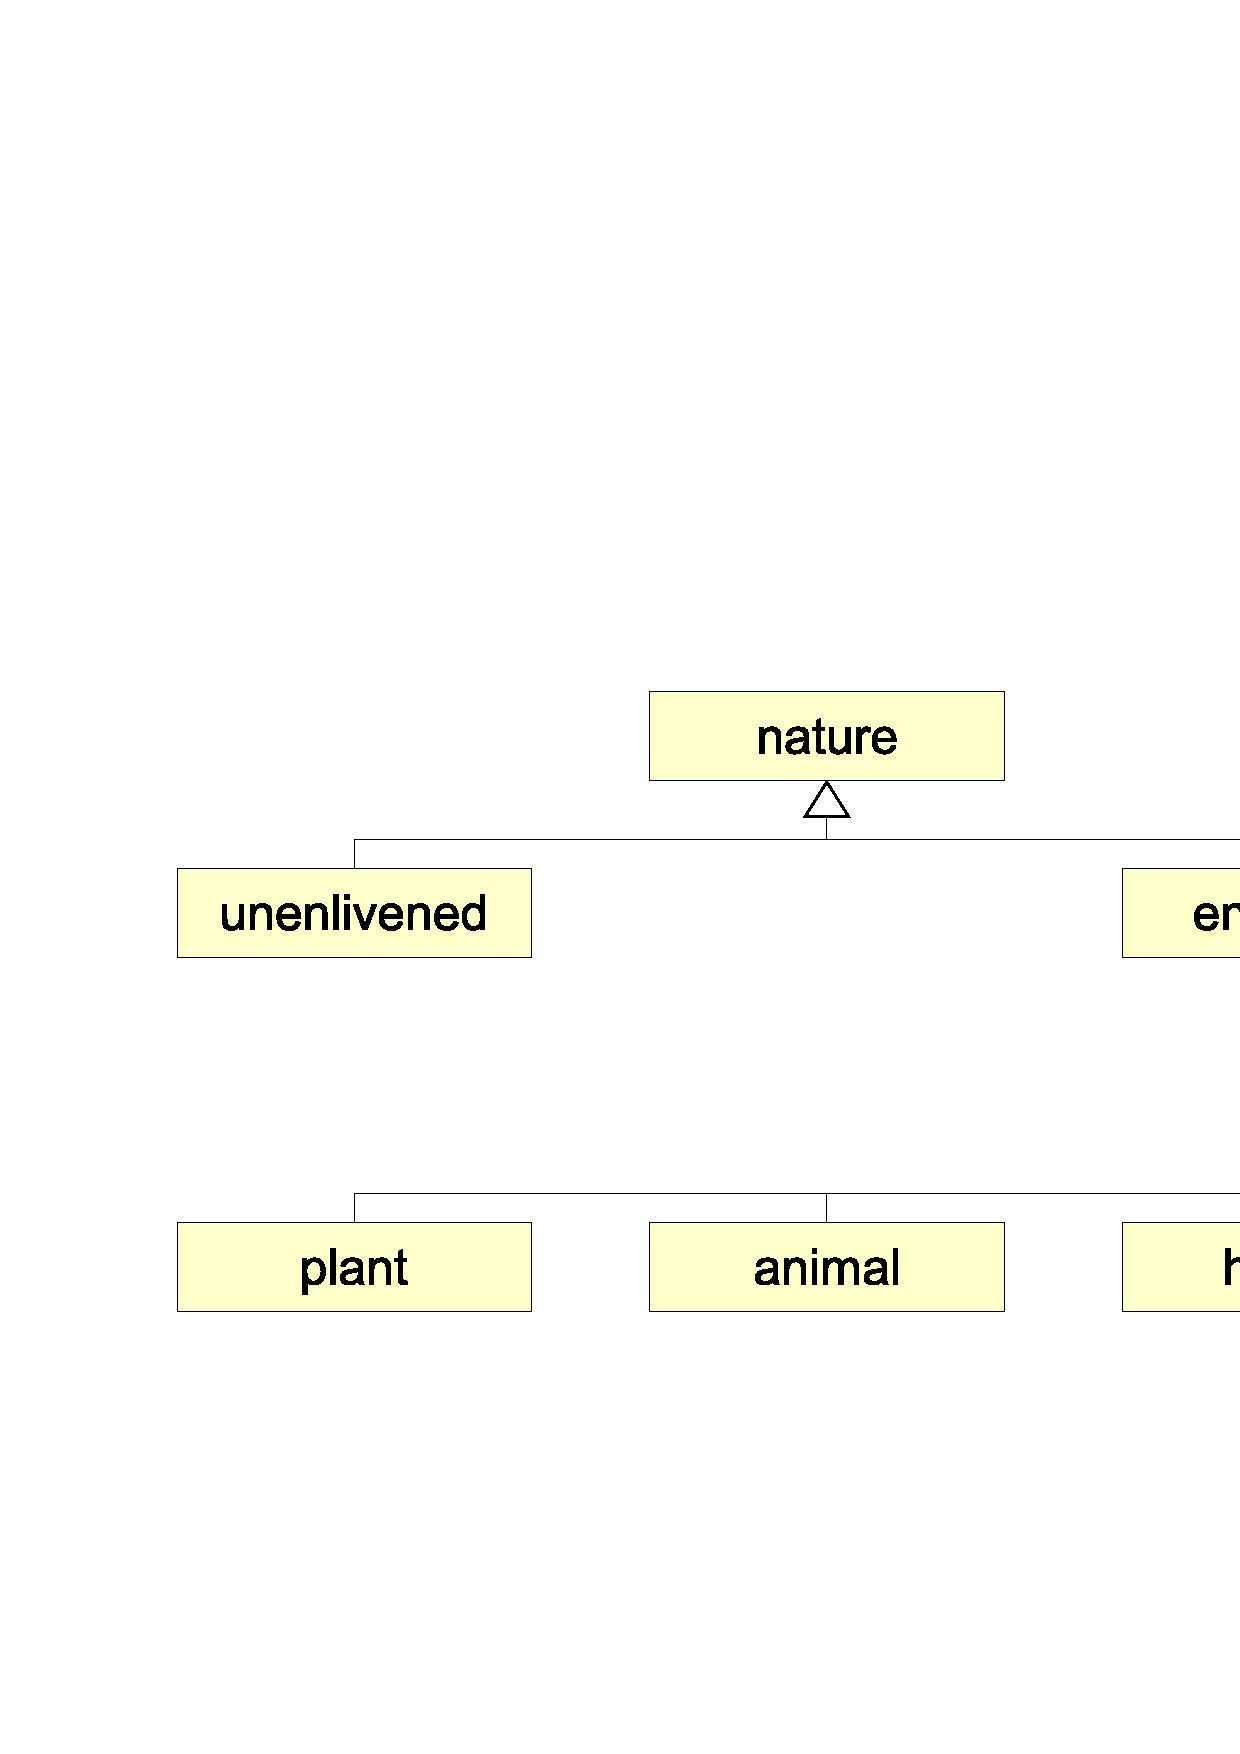
\includegraphics[scale=0.3,angle=-90]{graphic/nature.pdf}
        \caption{Systematics of Nature}
        \label{nature_figure}
    \end{center}
\end{figure}

This kind of classification stems from the earliest days of ancient science.
\emph{Plato}'s (429-347 B.C.) pupil \emph{Aristotle} (384-322 B.C.), being the
teacher of \emph{Alexander the Great}, was the first philosopher who logically
captured and organised the world. It was him who sorted items into clear groups
which he called \emph{Categories}. And it was him who first distinguished
between \emph{enlivened} and \emph{unenlivened} nature; who parted living forms
into \emph{Plants}, \emph{Animals} and \emph{Humans}. The science of biology
calls this classification a \emph{Systematics} (figure \ref{nature_figure}).

\emph{Categorisation} (classification) can be seen from two sides, depending on
what direction of that relationship one wants to emphasise. Taking Aristotle's
examples, \emph{Living Thing} would be a \emph{Generalisation} of \emph{Plants},
\emph{Animals} and \emph{Humans}. \emph{Animal} would be a \emph{Specialisation}
of \emph{Living Thing}.

Software developers often call categorisation an \emph{is-a} relationship and
talk of \emph{Super} and \emph{Sub} categories (sometimes also \emph{Parent}
and \emph{Child} categories). Section \ref{inheritance_heading} described how
\emph{Object Oriented Programming} (OOP) uses categorisation to let a sub class
inherit attributes and methods from its super class.
